\documentclass{standalone}
\usepackage{tikz}
\usetikzlibrary{calc}

\begin{document}

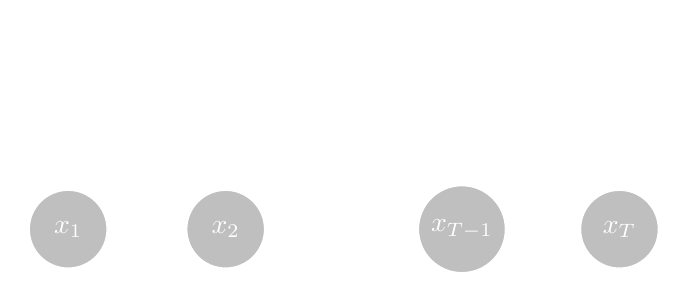
\begin{tikzpicture}[scale=1.5, node distance=2cm, every node/.style={circle, draw=white, text=white, minimum size=1cm, thick}, every path/.style={thick, white}]

    % Nodes
    \node[circle, draw=white] (yt1) {$y_1$};
    \node[circle, draw=white, right of=yt1] (yt) {$y_2$};  % Add spacing here with xshift
    \node[circle, draw=white, right of=yt, xshift=1cm] (yT1) {$y_{T-1}$};  % Add more spacing
    \node[circle, draw=white, right of=yT1] (yT) {$y_{T}$};  % Add more spacing
    
    \node[circle, draw=white, fill=gray!50, below of=yt1] (xt1) {$x_1$};
    \node[circle, draw=white, fill=gray!50, below of=yt] (xt) {$x_2$};
    \node[circle, draw=white, fill=gray!50, below of=yT1] (xT1) {$x_{T-1}$};
    \node[circle, draw=white, fill=gray!50, below of=yT] (xT) {$x_{T}$};
    
    % Edges with filled squares
    \draw[->] (yt1) -- (yt);
    \draw[->] (yt1) -- (xt1);
    \draw[->] (yt) -- (xt);
    \draw[->] (yT1) -- (xT1);
    \draw[->] (yT1) -- (yT);
    \draw[->] (yT) -- (xT);


    % Ellipsis for continuation
    \node[draw=none, fill=none] at ($(yt)!0.5!(yT1)$) {$\dots$};  % Three dots between yt and ytp1
    \node[draw=none, fill=none] at ($(xt)!0.5!(xT1)$) {$\dots$};  % Three dots between xt and xtp1

\end{tikzpicture}

\end{document}
